\documentclass[UTF8,a4paper]{article}
\usepackage{ctex}
\usepackage{amsmath}
\usepackage{amssymb}
\usepackage{graphicx}
\usepackage{fancyhdr}
\usepackage{CJK}
\usepackage{chngpage}
\usepackage{url}
\setCJKmainfont{宋体}
\usepackage{listings}
\usepackage{xcolor}
\usepackage[numbers,sort&compress]{natbib}
\usepackage{xpatch}
\usepackage{geometry}
\xpatchcmd{\thebibliography}{\section*}{\section}{}{}
\geometry{left=2.9cm,right=2.9cm,top=3cm,bottom=2.9cm}

\definecolor{CPPLight}  {HTML} {686868}
\definecolor{CPPSteel}  {HTML} {888888}
\definecolor{CPPDark}   {HTML} {262626}
\definecolor{CPPBlue}   {HTML} {4172A3}
\definecolor{CPPGreen}  {HTML} {487818}
\definecolor{CPPBrown}  {HTML} {A07040}
\definecolor{CPPRed}    {HTML} {AD4D3A}
\definecolor{CPPViolet} {HTML} {7040A0}
\definecolor{CPPGray}  {HTML} {B8B8B8}


\lstset{
	columns=fixed,       
	numbers=left,                                        % 在左侧显示行号
	frame=none,                                          % 不显示背景边框
	backgroundcolor=\color[RGB]{245,245,244},            % 设定背景颜色
	keywordstyle=\color[RGB]{40,40,255},                 % 设定关键字颜色
	numberstyle=\footnotesize\color{darkgray},           % 设定行号格式
	commentstyle=\it\color[RGB]{0,96,96},                % 设置代码注释的格式
	basicstyle=\small,
	stringstyle=\rmfamily\slshape\color[RGB]{128,0,0},   % 设置字符串格式
	showstringspaces=false,                              % 不显示字符串中的空格
	language=c++,                                        % 设置语言
	morekeywords={alignas,continute,friend,register,true,alignof,decltype,goto,
		reinterpret_cast,try,asm,defult,if,return,typedef,auto,delete,inline,short,
		typeid,bool,do,int,signed,typename,break,double,long,sizeof,union,case,
		dynamic_cast,mutable,static,unsigned,catch,else,namespace,static_assert,using,
		char,enum,new,static_cast,virtual,char16_t,char32_t,explict,noexcept,struct,
		void,export,nullptr,switch,volatile,class,extern,operator,template,wchar_t,
		const,false,private,this,while,constexpr,float,protected,thread_local,
		const_cast,for,public,throw,std},
	emph={map,set,multimap,multiset,unordered_map,unordered_set,
		unordered_multiset,unordered_multimap,vector,string,list,deque,
		array,stack,forwared_list,iostream,memory,shared_ptr,unique_ptr,
		random,bitset,ostream,istream,cout,cin,endl,move,default_random_engine,
		uniform_int_distribution,iterator,algorithm,functional,bing,numeric,},
	emphstyle=\color{CPPViolet}, 
}



%opening
\title{实验四 Hash函数MD5}
\author{1611531-信息安全-刘新慧}
\date{}
\begin{document}

\maketitle

\begin{abstract}
通过实际编程了解MD5算法的过程,加深对Hash函数的认识。\par 
\end{abstract}
\tableofcontents
\newpage

	\section{实验原理}
Hash函数是将任意长的数字串转换成一个较短的定长输出数字串的函数,输出的结果称为Hash值。Hash函数具有如下特点:\par
(1)	快速性:对于任意一个输入值x,由Hash函数 ,计算Hash值y,即 是非常容易的。\par 
(2)	单向性:对于任意一个输出值y,希望反向推出输入值x,使得 ,是非常困难的。\par 
(3)	无碰撞性:包括强无碰撞性和弱无碰撞性,一个好的Hash函数应该满足强无碰撞性,即找到两个不同的数字串x和y,满足 ,在计算上是不可能的。\par 
Hash函数可用于数字签名、消息的完整性检验。消息的来源认证检测等。
现在常用的Hash算法有MD5、SHA-1等。下面从MD5入手来介绍Hash算法的实现机制。\par 
MD系列单向散列函数是由Ron Rivest设计的,MD5算法对任意长度的输入值处理后产生128位的Hash值。MD5算法的实现步骤如下(见表4-1):\par 
	\begin{figure}[!ht]
	
	\centering
	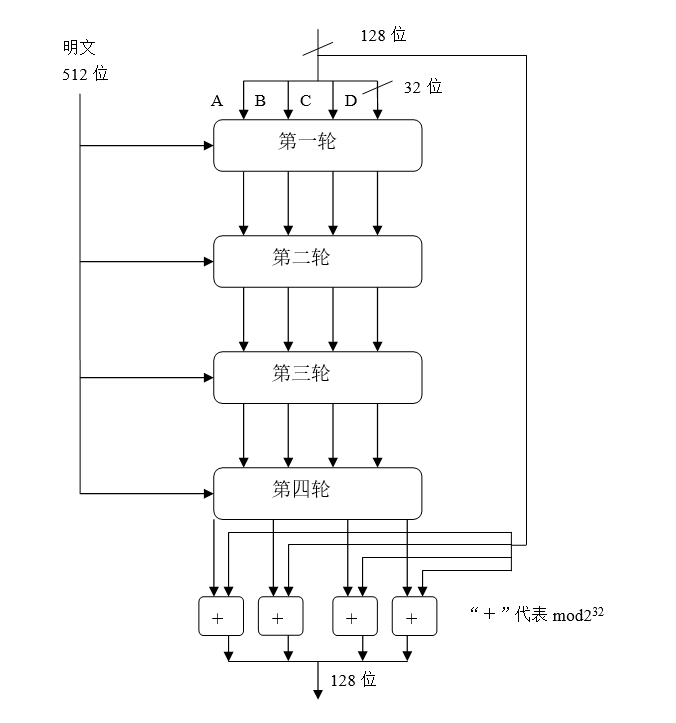
\includegraphics[width=0.67\textwidth]{table1.PNG}
	\caption{表4-1}
	\label{fig:table1}
\end{figure}
在MD5算法中,首先需要对信息进行填充,使其字节长度与448模512同余,即信息的字节长度扩展至 ,n为一个正整数。填充的方法如下:在信息的后面填充第一位为1,其余各位均为0,直到满足上面的条件时才停止用0对信息的填充。然后,再在这个结果后面附加一个以64位二进制表示的填充前信息长度。经过这两步的处理,现在的信息字节长度为 ,即长度恰好是512的整数倍,这样做的目的是为了满足后面处理中对信息长度的要求。\par 
MD5中有A、B、C、D,4个32位被称为链接变量的整数参数,它们的初始值分别为:\par 
A0=0x01234567,B0=0x89abcdef, C0=0xfedcba98, D0=0x76543210\par 
当设置好这4个链接变量后,就开始进入算法的4轮循环运算。循环的次数是信息中512位信息分组数目。\par 
首先将上面4个链接变量复制到变量A、B、C、D中,以备后面进行处理。\par 
然后进入主循环,主循环有4轮,每轮循环都很相似。第一轮进行16次操作,每次操作对A、B、C、D中的3个做一次非线性函数运算,然后将所得结果加上第四个变量,文本的一个子分组(32位)和一个常数。再将所得结果向左循环移S位,并加上A、B、C、D其中之一。最后用该结果取代A、B、C、D其中之一。\par 
 以下是每次操作中用到的4个非线性函数(每轮一个)。\par 

\begin{centering}
	$ 
	F(B,C,D)=(B\wedge C)\vee(\overline B\wedge D)
	$\par 
	$
		G(B,C,D)=(B\wedge D)\vee(C\wedge \overline D)
	$\par 
	$
		H(B,C,D)=B\oplus C\oplus D
	$\par 	
	$
		I(B,C,D)=C\oplus ( B\vee\overline D)
	$\par 
	
	\end{centering}

 MD5轮主要操作为:\par 
\begin{centering}
$a=b+((a+f(b,c,d)+M+t)<<<s)$



	\end{centering}
  对应于四轮操作,f分别取F,G,H,I;对每一轮的16次运算,M分别取M1,M2,…,M16。对于4轮共64次运算,t为给定的一些常数,另外一个常数 是 的整数部分,其中i=1,2,…,64。在 中,i的单位是弧度,由此构成了32位的随机数源 ,它消除了输入数据中任何规律性的特征。\par 
对于4轮64次操作的具体运算,可查阅课本的内容。所有这些操作完成之后,将A,B,C,D分别加上A0,B0,C0,D0。然后用下一分组数据继续进行运算,最后得到一组A,B,C,D。把这组数据级联起来,即得到128比特的Hash结果。\par 


	\section{实验内容和步骤}
1、	算法分析\par 
参照教材内容,分析MD5算法实现的每一步原理。\par 
2、	算法实现:\par 
利用Visual C++语言,自己编写MD5的实现代码,并检验代码实现的正确性。\par 
3、	雪崩效应检验:\par 
尝试对一个长字符串进行Hash运算,并获得其运算结果。对该字符串进
行轻微的改动,比如增加一个空格或标点,比较Hash结果值的改变位数。进行8次这样的测试。\par 
 



	\section{实验结果}
	\subsection{程序框图}
	程序框图如下:\par \newpage
	\begin{figure}[!ht]
		
		\centering
		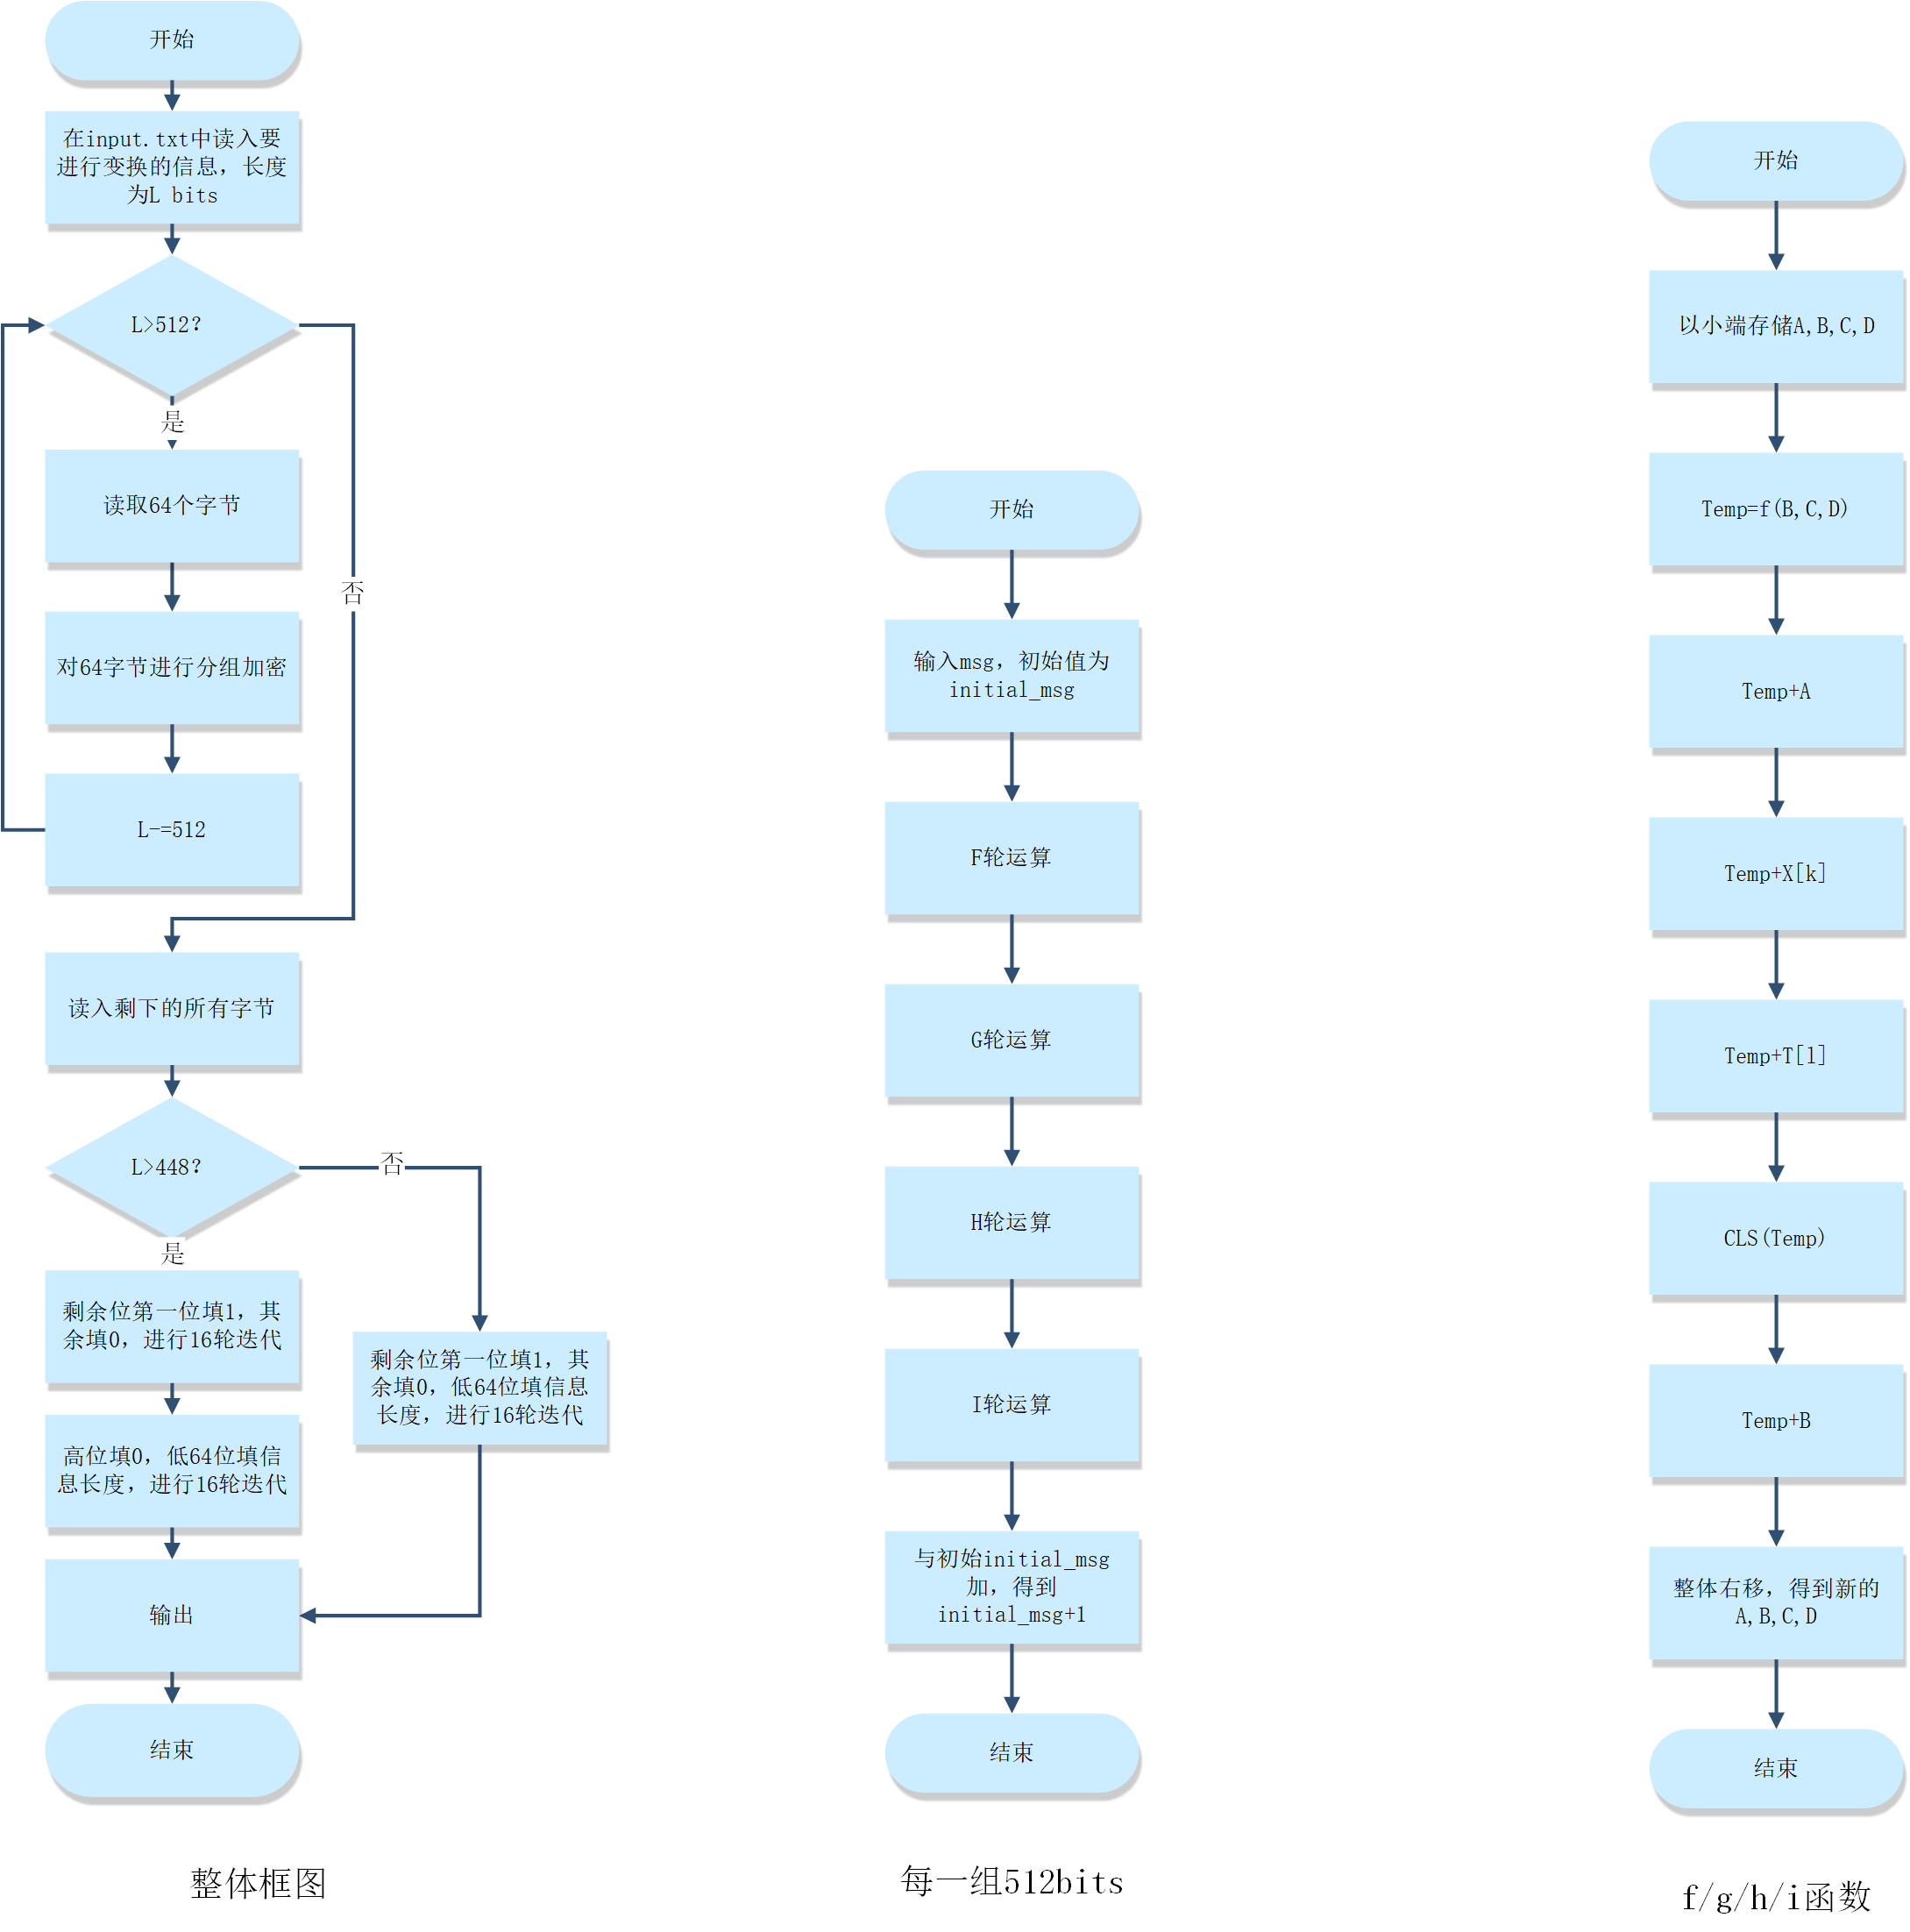
\includegraphics[width=0.8\textwidth]{liucheng.PNG}
	
		\label{fig:p3}
	\end{figure}
	
\subsection{实现MD5编程}	
运行代码以下为两个结果示例:\par 
当输入的内容为"a"时,结果如下:\par 
\begin{figure}[!ht]
	
	\centering
	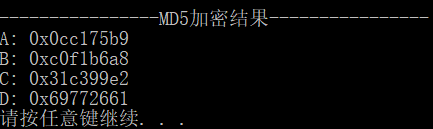
\includegraphics[width=0.8\textwidth]{r2.PNG}
	\caption{结果1}
	\label{fig:p3}
	\end{figure}
运行代码,当输入的内容为"ABCDEFGHIJKLMNOPQRSTUVWXYZabcdefghijklmnopqrs\par 
tuvwxyz0123456789"时,结果如下:\par 
\begin{figure}[!ht]
	
	\centering
	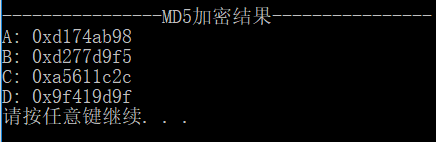
\includegraphics[width=0.8\textwidth]{r1.PNG}
	\caption{结果2}
	\label{fig:p3}
\end{figure}
\newpage
\subsection{雪崩效应}	
最开始进行hash的输入:Hello I am Lethe\par 

hash结果:0x03319a22f0416ae301a35743bf5d6ba6\par 

(1)输入修改为:H ello I am Lethe\par 
hash结果为:0x6947163a0a45ff14decaa73b8efd81b0\par 
改变位数为:64\par 



(2)输入修改为:He llo I am Lethe

hash结果为:0x033ab41e2d0c5d8fcf65d214eaa0c836\par 
改变位数为:64\par 



(3)输入修改为:Hel lo I am Lethe\par 
hash结果为:0xfab7e9a9cc2b32a14e416748547a1dca\par 
改变位数为:64\par 



(4)输入修改为:Hell o I am Lethe\par 
hash结果为:0xf04239ab5c01b72d38eb5222051ae388\par 
改变位数为:60\par 



(5)输入修改为:Hello I a m Lethe\par 
hash结果为:0xdb03fd0a6fa73873b63476b23b91c479\par 
改变位数为:67\par 



(6)输入修改为:Hello I am L ethe\par 
hash结果为:0x9a128057a978d32be86476a0b64f0157\par 
改变位数为:61\par 



(7)输入修改为:Hello I am Le the\par 
hash结果为:0xacb71a03f8e71d32510221fe90f2d556\par 
改变位数为:64\par 



(8)输入修改为:Hello I am Let he\par 
hash结果为:0x2c6f9f06bd86f0d1e951ce8c816ca7e8\par 
改变位数为:65\par 


平均结果为:(64+64+64+60+67+61+64+65)/8=63.625$\approx$64位\par 
\end{document}
